\subsubsection{Text Chat}
Sơ đồ use-case Text chat:
\begin{figure}[H]
    \centering
    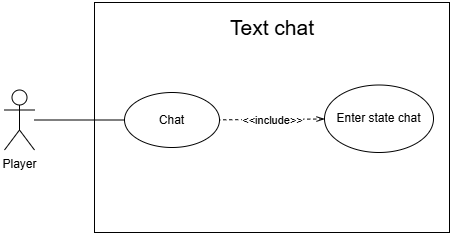
\includegraphics[width=0.75\linewidth]{4.Đặc tả chi tiết các lược đồ/Use-case/images/TextChat.png}
    \caption{Use-case mô tả Text Chat}
    \label{fig:placeholder}
\end{figure}


\begin{table}[H]
\centering
\begin{tabular}{|p{4cm}|p{10cm}|}
\hline
\textbf{Use-case name} & Text chat \\ \hline
\textbf{Actor} & Người chơi \\ \hline
\textbf{Descriptions} & Use-case này sẽ chỉ ra các bước cần thực hiện để có thể sử dụng text chat được. \\ \hline
\textbf{Pre-conditions} & Phải vào được trong lobby \\ \hline
\textbf{Trigger} & Không có. \\ \hline
\textbf{Post-conditions} & Không có \\ \hline
\textbf{Normal Flow} &
\begin{enumerate}
\item Người chơi nhấn phím ''Enter'' để vào chế độ chat.
\item Người chơi bắt đầu ghi các tin nhắn mong muốn.
\item Người chơi nhấn phím ''Enter'' để gửi tin nhắn.
\item Use-case kết thúc sau khi người chơi nhấn phím ''Enter'' để thoát khỏi chế độ chat.
\end{enumerate}
\\ \hline
\textbf{Alternative Flow} &
Không có
\\ \hline
\textbf{Exception Flow} &
Không có
\\ \hline
\end{tabular}
\end{table}